\documentclass{templateNote}
\usepackage{tcolorbox}
\usepackage{hyperref}
\usepackage{amsmath}
\usepackage{amssymb}

\begin{document}

\imagenlogoU{img/LogoElNube.png}
\linklogoU{https://github.com/MarceloPazPezo}
\linkQRDoc{https://github.com/MarceloPazPezo/MyRepo/tree/main/Icinf}
\titulo{Test 1}
\asignatura{Gestión Presupuestaria y Financiera}
\autor{
    \indent
    Marcelo \textsc{Paz}
}

\vDoc{1.0.0}
\portada
\margenes % Crear márgenes

\section{Conceptos Claves}
\begin{itemize}
    \item \textbf{Interés Simple.}
    \item \textbf{Interés Compuesto.}
    \item \textbf{Criterios de Evaluación.}
    \begin{itemize}
        \item Valor Actual (VA)
        \item Valor Actual Neto (VAN)
        \item Valor Cuota (VC)
        \item Carga Anual Equivalente (CAE)
    \end{itemize}
    \item \textbf{Análisis del balance general.}
    \item \textbf{Análisis del estado de resultados.}
    \item \textbf{Análisis del estado de flujo de efectivo.}
    \item \textbf{Aplicación de índices financieros.}
    \item \textbf{Pronóstico de ventas.}
    \item \textbf{Estados finacieros proyectados.}
    \item \textbf{Bonos y acciones.}
    \item \textbf{Valor par, valor sobre la par y valor.}
    \item \textbf{Acciones Preferentes.}
    \item \textbf{Autofinanciación.}
\end{itemize}

\section{Bibliografia}
\begin{itemize}
    \item Van Horne, J. y Wachowicz, J. (2002). Fundamentos de Administración Financiera (11ª ed.): Prentice-Hall.
    \item Díaz, V. (1995). Matemáticas Financieras (2ª ed.): McGraw-Hill.
    \item Welsch, G., Hilton, R. y Gordon, P. (1990). Presupuestos, Planificación y Control de Utilidades (5ª ed.): Prentice Hall
\end{itemize}

\section{Apunte}
\subsection*{Interés Simple:}
Es el interés que se paga sobre el capital inicial.
\begin{itemize}
    \item El capital inicial se mantiene igual durante toda la operación.
    \item El interés es el mismo para cada uno de los períodos de la operación.
    \item La tasa de interés se aplica sobre el capital invertido o capital inicial.
\end{itemize}
\begin{figure}[H]
    \centering
    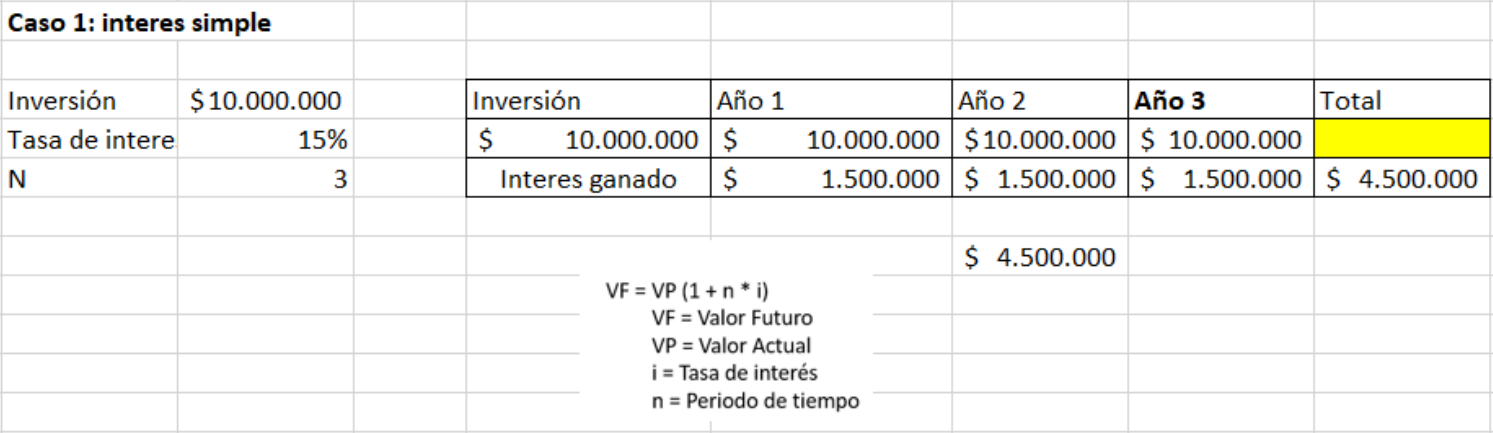
\includegraphics[width=1\textwidth]{img/InteresSimple.png}
    \caption{Interés Simple}
\end{figure}

\subsection*{Interés Compuesto:}
Es el interés que se paga sobre el capital inicial más los intereses acumulados.
\begin{itemize}
    \item El capital inicial aumenta en cada periodo debido a que los intereses se van sumando.
    \item La tasa de interés se aplica sobre un capital que va variando.
    \item Los intereses son cada vez mayores.
\end{itemize}
\begin{figure}[H]
    \centering
    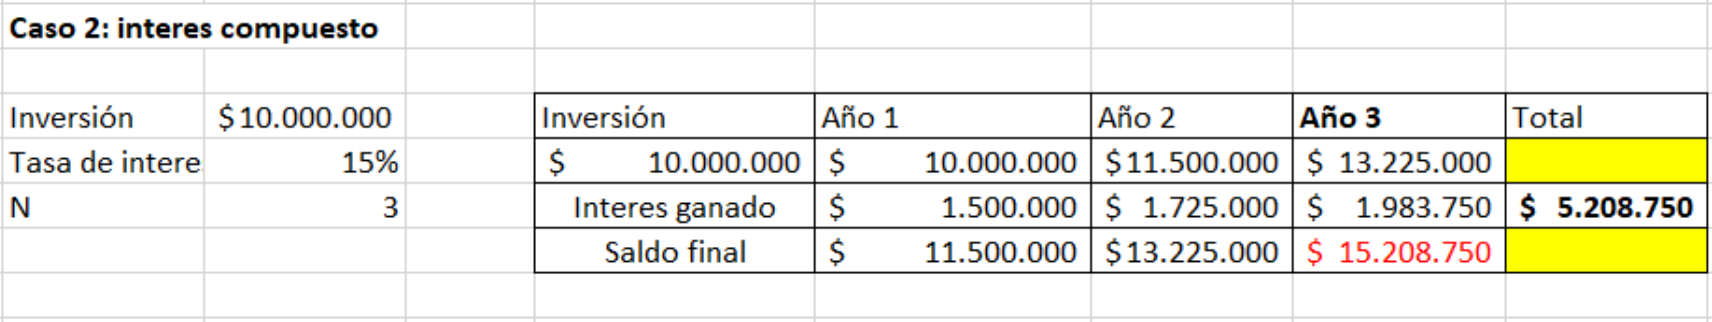
\includegraphics[width=1\textwidth]{img/InteresCompuesto.png}
    \caption{Interés Compuesto}
\end{figure}

\newpage
\subsection*{Costo de Oportunidad:}
\begin{itemize}
    \item \textbf{Criterios de decisión}
    \begin{itemize}
        \item Si la rentabilidad del proyecto $ > $ Costo de oportunidad $\Rightarrow$ El proyecto es rentable.
        \item Si la rentabilidad del proyecto $ < $ Costo de oportunidad $\Rightarrow$ El proyecto no es rentable.
        \item Si la rentabilidad del proyecto $ = $ Costo de oportunidad $\Rightarrow$ El proyecto es indiferente.
    \end{itemize}
\end{itemize}
\begin{figure}[H]
    \centering
    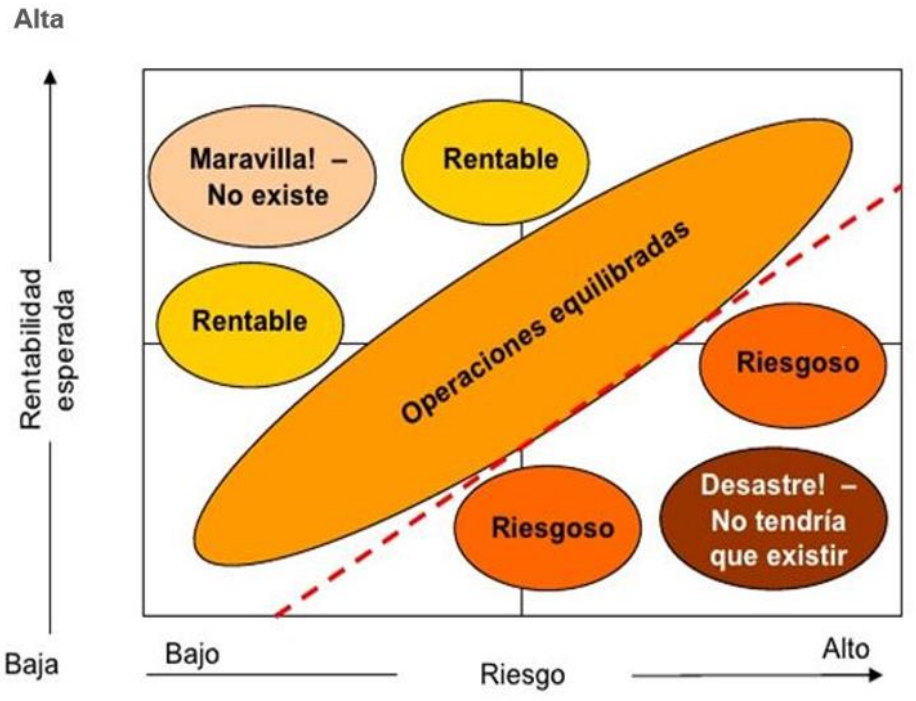
\includegraphics[width=1\textwidth]{img/Criterios.png}
\end{figure}

\subsection*{Tasa de rendimiento}
La tasa de rendimiento sobre la inversión es la ganancia en proporción del desembolso inicial.
\begin{equation*}
    \text{Tasa de rendimiento} = \frac{\text{Ganancia}}{\text{Inversión}} \times 100\%
\end{equation*}
\textbf{Regla de la tasa de rendimiento.} Aceptar inversiones que ofrezcan tasas de rendimiento que superen sus costos de oportunidad del capital.

\newpage
\subsection*{Valor Futuro}
Corresponde al valor que tendría un capital actual, colocado a una cierta tasa de interés, por unu alpso de ciertos períodos, al final de dichos períodos. Es aquella idea que persigue un inversionista de invertir el día de hoy para obtener un rendimiento en el futuro.
\begin{equation*}
    \text{VF} = \text{VP} \times (1 + i)^n
\end{equation*}
Donde:
\begin{itemize}
    \item VF: Valor Futuro.
    \item VP: Valor presente (Capital inicial).
    \item i: Tasa de interés.
    \item n: Número de períodos.
\end{itemize}

\subsection*{Valor Presente}
Es el que corresponde a un bien, una inversión, cantidad de dinero o un valor
en un instante considerado como presente, lo que permite evaluar su equivalencia con
otros bienes, valores o inversiones.
\begin{equation*}
    \text{VP} = \frac{\text{VF}}{(1 + i)^n}
\end{equation*}
Donde:
\begin{itemize}
    \item VF: Valor Futuro.
    \item VP: Valor presente (Capital inicial).
    \item i: Tasa de interés.
    \item n: Número de períodos.
\end{itemize}

\subsection*{Valuacion de flujos de efectivo en varios periodos}
\textbf{Flujo de efectivo descontado (FED)}, se abrevia como:
\begin{equation*}
    \text{VP} = \sum_{t=0}^{n} \frac{{VF}_t}{(1 + i)^t}
\end{equation*}

\newpage
\subsection*{Valor Actual Neto (VAN)}
Son los flujos descontados menos la inversión.
Si el VAN es mayor a cero se realiza la inversión.
\begin{equation*}
    \text{VAN} = \sum_{t=0}^{n} \frac{{VF}_t}{(1 + i)^t} - I_0
\end{equation*}
Donde:
\begin{itemize}
    \item ${VF}_t$: Valor futuro.
    \item $I_0$: Inversión inicial.
    \item $i$: Tasa de descuento.
    \item $t$ : Periodo.
\end{itemize}
\begin{equation*}
    \scalebox{0.8}{$\text{VAN del Activo} = \text{VP de los flujos de efectivo esperados futuros} - \text{Costo del activo}$}
\end{equation*}
\begin{equation*}
    \scalebox{0.8}{$\text{VAN} = \text{Cual es el valor del activo} - \text{Cual es su costo}$}
\end{equation*}

\begin{itemize}
    \item VAN $ > 0$: Crea valor.
    \item VAN $ < 0$: Destruye valor.
    \item VAN $ = 0$: Punto de equilibrio.
\end{itemize}
\textbf{Inconvenientes del VAN:}
\begin{enumerate}
    \item No tiene en cuenta el cambio del valor del dinero a lo largo del tiempo debido a la inflación y los tipos de interés.
    \item No tiene en cuenta los ingresos producidos despues del plazo de recuperación, lo que lleva a primar inversiones de corta duración o con altos flujos de caja al principio del proyecto.
    \item Es necesario hacer una previsión de los flujos de caja futuros. \textbf{¿Cómo voy a saber exactamente la cantidad de dinero que me va a permitir obtener una inversión?}
    \item Prima la liquidez sobre la rentabilidad, es decir, tienen prioridad los proyectos que me permiten recuperar mi inversión lo antes posible, frente a otros que pueden dar más rentabilidad en el futuro.
\end{enumerate}

\newpage
\subsection*{Tasa interna de retorno (TIR)}
\noindent
Es la tasa de descuento con la que el valor actual neto es igual a cero.
\begin{equation*}
    \text{VAN} = \sum_{t=0}^{n} \frac{F_t}{(1 + TIR)^t} - I_0 = 0
\end{equation*}
Donde:
\begin{itemize}
    \item $F_t$: Flujo de efectivo en el periodo t.
    \item $I_0$: Inversión inicial.
    \item $TIR$: Tasa interna de retorno.
    \item $t$ : Periodo.
\end{itemize}

\subsection*{Amortización}
Es el pago gradual de la deuda por la vía de una cuota con un interés fijo y un tiempo limitado.
\begin{equation*}
    \text{Cuota} = \frac{C \times i\%}{1 - \frac{1}{(1 + i\%)^{n}}}
\end{equation*}
Donde:
\begin{itemize}
    \item $C$: Credito.
    \item $i$: Tasa de interés.
    \item $n$: Número de periodos.
    \item $Cuota$: Pago mensual.
    % \item $\frac{1}{(1+i\%)^n}$: Factor de amortización.
\end{itemize}
\begin{figure}[H]
    \centering
    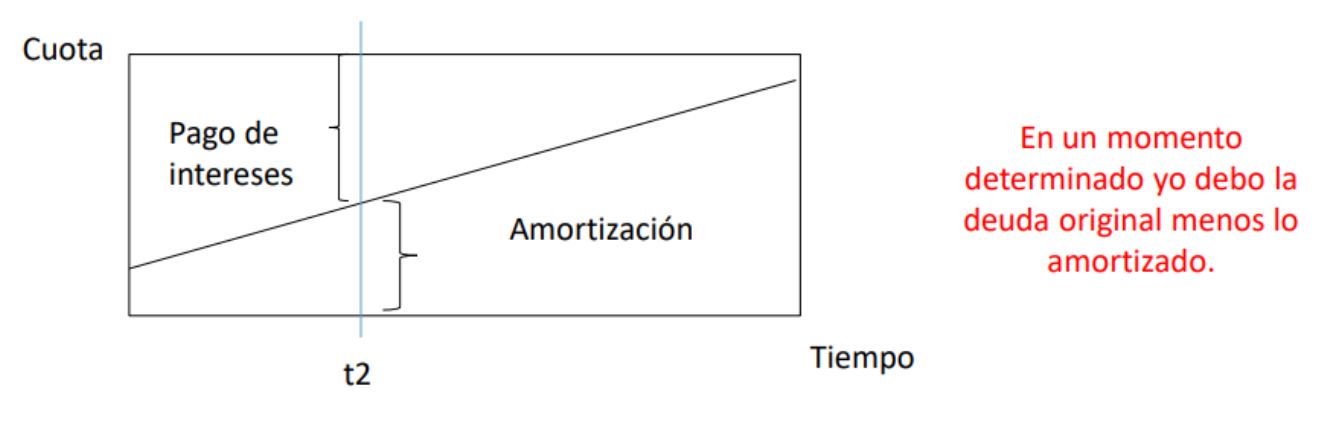
\includegraphics[width=1\textwidth]{img/Amortizacion.png}
\end{figure}

\subsection*{Tasa de interés equivalente}
Si se tiene una tasa de interés anual (IA), la tasa de interés mensual equivalente (IM), puede ser calculada usando:
\begin{equation*}
    \text{IM} = (1 + \text{IA})^{1/12} - 1 \times 100
\end{equation*}

\subsection*{Carga Anual Equivalente (CAE)}
\begin{itemize}
    \item La Carga Anual Equivalente (CAE) es un indicador porcentual, que incluye los intereses, gastos y seguros asociados al crédito expresados en forma anual que permiten comparar en forma objetiva el costo del crédito entre entidades.
    \item Mediante la CAE, las personas podrán comparar diferentes alternativas de crédito, sin importar las diferencias en las variables que cada entidad tenga establecidas.
    \item Una CAE menor es señal de que, financieramente, es la alternativa más conveniente, ya que considera todos los elementos del crédito.
\end{itemize}
\begin{equation*}
    \text{CAE} = (1+i_f)^n - 1
\end{equation*}
\end{document}